\documentclass[../TDE8_filtrage.tex]{subfiles}%

\begin{document}
\section[s]"1"{Lecture de diagrammes de \textsc{Bode}}
\enonce{%
	On donne Figure~\ref{fig:ddBIII} les diagrammes de \textsc{Bode} de quatre
	filtres.
	\begin{figure}[htbp!]
		\centering
		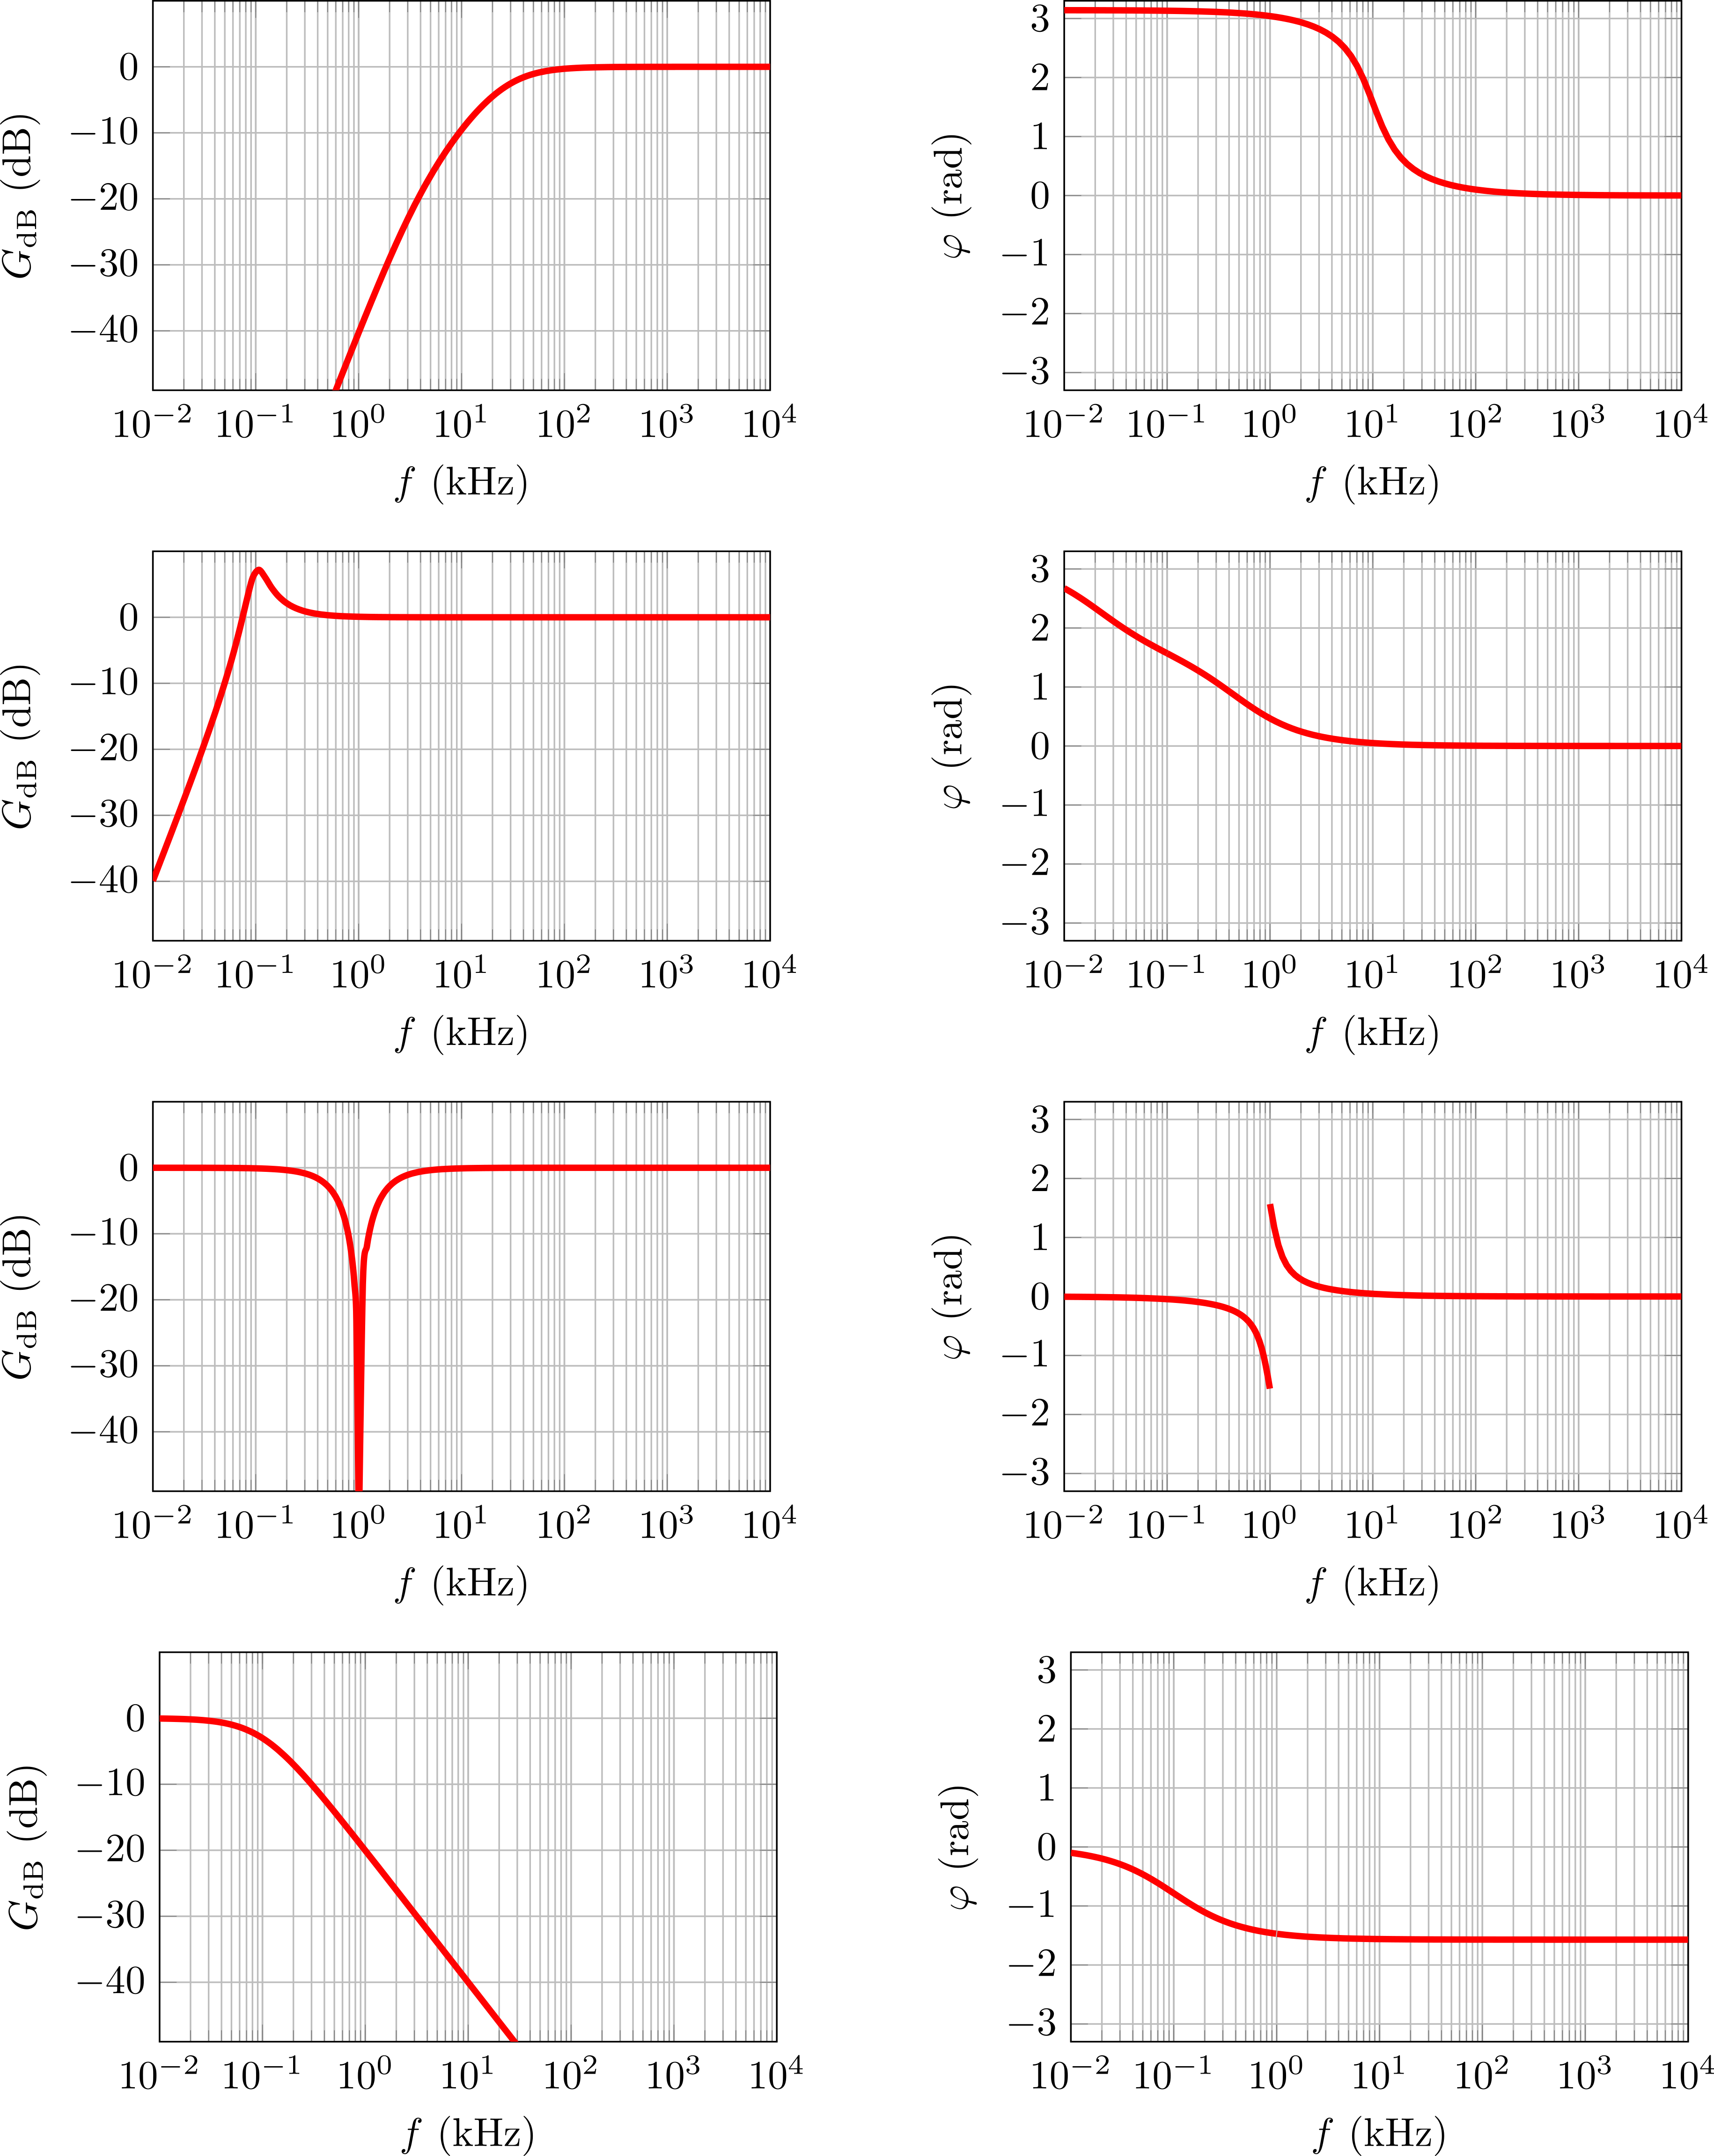
\includegraphics[scale=1]{bode_lect-plain}
		\caption{Diagrammes exercice III}
		\label{fig:ddBIII}
	\end{figure}
}
\QR{%
Pour chacun d'eux~:
\begin{enumerate}
	\item Indiquer le type de filtre dont il s'agit.
	\item Déterminer l'expression du signal $s(t)$ de sortie du filtre pour un
	      signal d'entrée
	      \[e(t) =
		      E_0 +
		      E_1\cos(\wt) +
		      E_{10}\cos \left( 10\wt + \frac{\pi}{4} \right) +
		      E_{100}\cos \left( 100\wt - \frac{\pi}{3} \right)
	      \]
	      avec une fréquence $f = \SI{1}{kHz}$
	      % et $E_0 = E_1 = E_{10} = E_{100} = \SI{5}{V}$.
\end{enumerate}
}{%
Pour faciliter la rédaction on note $e(t) = e_0 + e_1 (t) + e_{10} (t) + e_{100}
	(t)$, et de même pour le signal de sortie $s$. Ainsi, par linéarité, chaque
composante $e_n$ du signal d'entrée donne une composante $s_n$ au signal de
sortie.
\begin{itemize}
	\item Filtre 1~: d'après l'allure du diagramme de \textsc{Bode}, il s'agit d'un
	      filtre passe-haut, de fréquence de coupure $f_c$ de l'ordre de
	      \SI{10}{kHz}. Reconstruisons le signal de sortie~:
	      \begin{itemize}
		      \item Le terme constant $e_0$ est complètement coupé par le filtre,
		            donc $s_0 = 0$.
		      \item L'harmonique de fréquence $f$ est atténuée de \SI{40}{dB} et
		            peut donc être négligée dans le signal de sortie (\SI{40}{dB}
		            correspond à une division de l'amplitude par 100), soit $s_1 (t)
			            \ll$ autres harmoniques de $s(t)$.
		      \item L'harmonique de fréquence $10f$ est atténuée de \SI{10}{dB},
		            soit
		            \[S_{10} = 10^{-10/20} E_{10} = 10^{-1/2} E_{10} \approx \num{0,3}E_{10}\]
		            et
		            elle est également déphasée d'environ $+\pi/2$. Ainsi
		            \[s_{10} (t) \approx \num{0,3}E_{10} \cos(10\wt + \pi/4 + \pi/2)\]
		      \item L'harmonique de fréquence $100f$ n'est presque pas atténuée ni
		            déphasée, donc $s_{100} (t) \approx e_{100} (t)$. Au final, on
		            obtient le signal de sortie $s(t)$ suivant~:
	      \end{itemize}
\end{itemize}

\[\boxed{
	s(t) \approx
	\num{0,3}E_{10} \cos \left(10\wt + \frac{3\pi}{4}\right) +
	E_{100} \cos \left(100\wt - \frac{\pi}{3}\right)
	}\]

\begin{itemize}
	\item Filtre 2~: d'après l'allure du diagramme de \textsc{Bode}, il s'agit d'un
	      filtre \textbf{passe-haut}, de fréquence de coupure $f_c$ de l'ordre de
	      \SI{0.1}{kHz}. De la même manière que pour le fitre 1, on détermine que~:
\end{itemize}

\[\boxed{
		s(t) \approx
		E_1 \cos (\wt) + E_{10} \cos \left(10\wt + \frac{\pi}{4}\right) +
		E_{100} \cos \left(100\wt - \frac{\pi}{3}\right)
	}\]
\begin{itemize}
	\item Filtre 3~: d'après l'allure du diagramme de \textsc{Bode}, il s'agit d'un
	      filtre \textbf{coupe-bande}, la bande coupée étant proche de
	      \SI{1}{kHz}. Ainsi seule l'harmonique $e_1(t)$ est coupée (soit $s_1 =
		      0$). Les autres composantes harmoniques du signal d'entrée, y compris la
	      composante continue, sont de fréquences suffisamment différentes de la
	      fréquence coupée pour n'être ni atténuée ni déphasée. La signal de
	      sortie $s(t)$ s'écrit donc sous la forme~:
\end{itemize}

\[\boxed{
		s(t) =
		E_0 +
		E_{10} \cos \left(10\wt - \frac{\pi}{4}\right) +
		E_{100} \cos \left(100\wt - \frac{\pi}{3}\right)
	}\]
\begin{itemize}
	\item Filtre 4~: d'après l'allure du diagramme de \textsc{Bode}, il s'agit
	      d'un filtre \textbf{passe-bas}, de fréquence de coupure $f_c$ de l'ordre
	      de \SI{0.1}{kHz}. Le terme constant $e_0$ passe au travers du filtre
	      sans être modifié. Les termes suivants sont de fréquence suffisamment
	      supérieure à la fréquence de coupure pour que le diagramme de
	      \textsc{Bode} puisse être approximé par son asymptote. On peut alors
	      déterminer le signal de sortie comme dans le cas du premier filtre, mais
	      il y a plus simple~! Comme le filtre est d'ordre 1 (une seule asymptote
	      de pente \SI{-20}{dB/décade}, alors il se comporte comme un intégrateur
	      pour les signaux de fréquence supérieure à sa fréquence de coupure. En
	      déduire le signal de sortie est donc très simple~:
\end{itemize}

\[s(t) =
	E_0 +
	\frac{\w_c}{\w}E_1\sin(\wt) +
	\frac{\w_c}{10\w}E_{10}\sin \left( 10\wt + \frac{\pi}{4} \right) +
	\frac{\w_c}{100\w}E_{100}\sin \left( 100\wt - \frac{\pi}{3} \right)
\]
\begin{itemize}
	\item{}
	      En écrivant le signal en termes de cosinus, on obtient~:
\end{itemize}
\[\boxed{
	s(t) =
	E_0 +
	\frac{\w_c}{\w}E_0\cos\left(\wt - \frac{\pi}{2}\right) +
	\frac{\w_c}{10\w}E_{10}\cos \left( 10\wt - \frac{\pi}{4} \right) +
	\frac{\w_c}{100\w}E_{100}\cos \left( 100\wt - \frac{5\pi}{6} \right)
	}\]
}

\end{document}
